\chapter{Deployment on Mobile and Scalability}\label{ch:deployment}
\section{What the measured prototype establishes}
The artifact executes a complete local pipeline, but its measured host behaviour does not support running full learned recognition on every display frame. The primary full pipeline has an isolated median query-and-render time of \LatencyFull{} ms on the recorded CPU configuration. Exhaustive learned matching takes \LatencyLocal{} ms, exhaustive SIFT takes \LatencyClassical{} ms, and global-only retrieval takes \LatencyRetrieval{} ms. These generated values describe different functionality, so the fast global result cannot be substituted for a complete anchored query.

\resultinput{profiles.tex}
\Cref{tab:profiles} includes upper-tail latency and process peak memory. The full learned path requires substantially more host resources than the classical recogniser. Reference caching reduces repeated work but also retains feature tensors. The process peak includes Python and library imports as well as weights and intermediate buffers; it is not a phone application memory estimate.

\begin{figure}[htbp]\centering
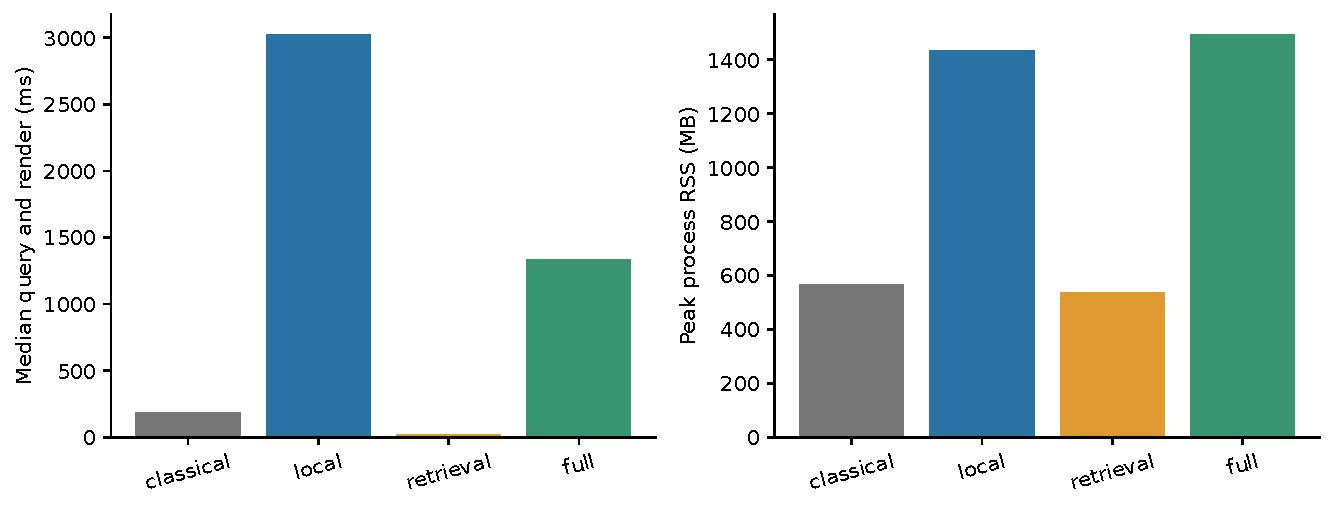
\includegraphics[width=\textwidth]{efficiency.pdf}
\caption{Measured isolated host query latency and complete-process peak RSS. Reference features are cached and query images are predecoded. The global-only path does not perform geometric anchoring.}\label{fig:efficiency}
\end{figure}
\Cref{fig:efficiency} supports the main deployment conclusion: a useful mobile design should decouple occasional recognition from continuous native tracking. This is a design implication of the measured workload, not a claim that such a phone integration has been completed. The original tracking script's faster frame average in \cref{tab:originals} illustrates the distinction between finding a target and maintaining an already acquired relation.

\section{Executed ONNX export}
The CosPlace global model was exported to a fixed-input ONNX graph and checked with the ONNX validator. The graph uses the same learned weights and descriptor normalisation as native PyTorch. Float ONNX outputs were compared with native descriptors on the actual downloaded Tokyo images. The observed maximum absolute difference is recorded in \cref{tab:exports}; it is sufficiently small for the float retrieval rankings in this run to match the native results.

\resultinput{exports.tex}
The export scope is deliberately narrow: it covers the global descriptor, not SuperPoint, LightGlue, RANSAC, rendering, or a complete camera application. A successful descriptor graph does not establish that dynamic keypoint operations and adaptive matching export without changes. Nor does graph validation prove that a chosen mobile execution provider supports every operator efficiently. No TFLite, CoreML or phone-native full-pipeline artifact is claimed.

The executed float graph is \FpModelMB{} MB and has median descriptor inference of \FpLatency{} ms in the recorded ONNX Runtime CPU test. This timing excludes image preprocessing and gallery search. It also differs from the separate native global query profile because the runtime, timed work and query population differ. The thesis retains these definitions rather than combining the faster number from one test with the broader functionality of another.

\section{Executed INT8 quantisation}
\subsection{Calibration and graph form}
Static quantisation used QDQ graph representation with a calibration reader drawn only from the reserved HPatches training places. Convolution and supported linear operators were selected for quantisation; remaining operations continue in floating point. The model is therefore a mixed graph with INT8-weight and activation paths, not a claim that every computation uses integer arithmetic. ONNX Runtime documents the distinction between graph representations and quantisation settings \citep{onnxquant}.

In a generic affine quantiser, a real value $x$ is mapped to
\begin{equation}
 q=\operatorname{clip}\bigl(\operatorname{round}(x/s)+z,q_{\min},q_{\max}\bigr),
 \qquad \widehat x=s(q-z),
\end{equation}
where $s$ is a scale and $z$ a zero point. Calibration estimates ranges for the selected activations. This introduces approximation error and possible saturation; a successful graph conversion alone cannot establish preservation of descriptor rankings. The artifact consequently performs actual quantised inference and retrieval evaluation.

\subsection{Measured size, latency and accuracy}
The executed quantised graph occupies \IntModelMB{} MB and has median descriptor inference of \IntLatency{} ms in the recorded CPU test. Both reductions are measured from produced files and runtime calls. Descriptor parity error is larger than for the float graph, as expected from the approximation, but the practical consequence must be read from retrieval rather than from an arbitrary tolerance alone.

\begin{figure}[htbp]\centering
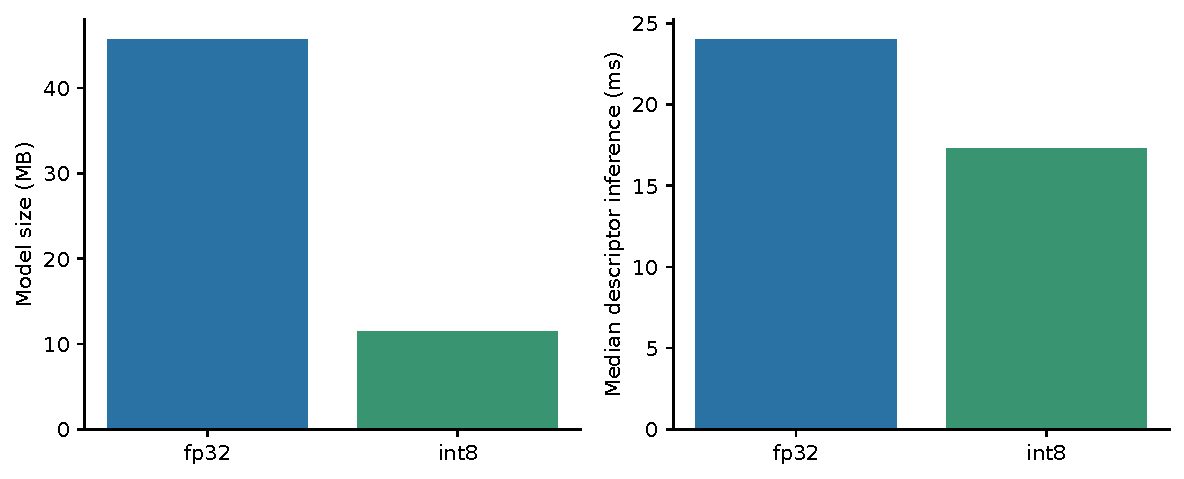
\includegraphics[width=\textwidth]{quantization.pdf}
\caption{Actual global-descriptor ONNX file size and CPU inference after QDQ quantisation. These measurements exclude the local matcher and do not represent an end-to-end phone speedup.}\label{fig:quantization}
\end{figure}
\resultinput{quant-retrieval.tex}
\Cref{fig:quantization,tab:quant-retrieval} show the trade-off. The aligned cross-time subsets retain their observed saturated retrieval, but the difficult daytime viewpoint split changes ranking accuracy. Thus quantisation is not accuracy-free even though several protocol scores remain unchanged. Calibration on training scenes also leaves an appearance-domain mismatch with Tokyo, which a broader deployment study should investigate.

The global encoder is only one part of the full query cost. Reducing it cannot remove the much larger local extraction and matching workload observed in the host profile. The descriptor export is still useful because it produces a concrete deployment candidate and reduces storage, but it does not establish that the full learned AR pipeline meets an interactive frame budget.

\section{Recognition and tracking schedules}
\designnote
A proposed mobile state machine has unlocalised, searching, verified and tracking states. Searching invokes retrieval and local verification. A verified observation establishes a relation to the stored place representation. A native visual-inertial tracker then propagates the camera pose at the platform's tracking rate. Loss of tracking, large uncertainty, or an elapsed refresh policy can trigger recognition again.

This design separates two failure types. Recognition failure means no supported map relation was found. Tracking failure means the relation was previously known but current device motion can no longer be estimated reliably. Reusing the last recognition output indefinitely would conceal the second failure. Instead, anchor visibility should depend on current tracking quality and the age of the last verified relation.

The state machine would require explicit time accounting. If a recognition call takes $T_r$ and is requested at an interval $\Delta$, the average recognition workload scales with $T_r/\Delta$ when calls do not overlap. This expression is a scheduling model, not a measured battery result. A real implementation must also account for camera processing, graphics, model warmup, thermal throttling and concurrent native tracking.

\ifFullReport
\section{Coordinate integration with AR platforms}
A persistent world-space post requires a relation between the place map and the device's current tracking world. Let $T_{w\leftarrow m}$ map map coordinates into the local tracking world, and let $T_{m\leftarrow a}$ define the stored anchor. The rendered anchor relation is
\begin{equation}
 T_{w\leftarrow a}=T_{w\leftarrow m}T_{m\leftarrow a}.
\end{equation}
The matrix direction must be documented at the API boundary; otherwise an inverse or axis-convention error can produce a stable but incorrect pose. Camera intrinsics, image rotation and screen-to-camera transforms must also be handled consistently.

The current homography prototype supplies a reference-plane image relation rather than $T_{w\leftarrow m}$. A calibrated plane with known geometry could provide additional constraints, while a sparse map and PnP supply a more general route. Neither follows automatically from a retrieved photograph. This is the key missing integration between the implemented planar demo and the social concept's arbitrary three-dimensional objects.

ARCore Cloud Anchors and ARKit saved world maps provide relevant platform mechanisms for hosting or restoring spatial relations \citep{arcore,arkit}. Integrating either would require its current lifecycle and privacy requirements, plus on-device tests. Azure Spatial Anchors is not proposed as a new dependency because its retirement has been confirmed \citep{azure}. The architecture should avoid making long-lived content records depend exclusively on a service identifier that cannot be migrated.
\fi

\section{Reference coverage and GPS priors}
The Tokyo viewpoint failure suggests a reference-coverage problem as well as a representation problem. A single front-facing reference may share too little visual content with a side-facing query. A proposed place model should therefore retain several directions or local submaps. Additional references raise storage and matching costs, making the retrieval hierarchy more important. This collection strategy remains a hypothesis until evaluated with an expanded gallery.

If the user permits a coarse location prior, candidate retrieval could first restrict the map region. The visual score could be combined with a spatial prior schematically as
\begin{equation}
 S_i=\lambda s_i+(1-\lambda)\log P(p_i\mid\ell),
\end{equation}
where $\ell$ is the permitted location observation. The parameter $\lambda$ and prior model would need validation. The current experiments do not use GPS filtering, so their results cannot be attributed to such a prior.

Location filtering creates its own failure mode when a noisy or denied position excludes the correct place. A mobile client should support uncertainty-aware region expansion or a visual-only fallback. It should also avoid logging detailed movement simply to make retrieval convenient. The privacy analysis treats the prior as an optional input with a distinct retention policy.

\ifFullReport
\section{Descriptor and map storage}
For $M$ references and global dimension $d$, a dense descriptor matrix requires approximately $Mdb$ bytes when each value occupies $b$ bytes, before index metadata. Local storage adds keypoint coordinates, local descriptors and any associated 3D-point identifiers. The actual checkpoint and process-memory measurements show that model bytes alone are not the complete footprint.

The 128-dimensional projection experiment demonstrates one compact-descriptor route but does not establish its accuracy benefit. Quantised storage or dimensional reduction should be evaluated through retrieval recall and geometric success, not only compression ratio. Approximate search would add another accuracy-cost parameter. A scalable system should benchmark those parameters independently before combining them into a single efficiency claim.

Reference-feature caches also need an eviction policy. Keeping every reference tensor resident is feasible for this small artifact but not for a global application. A region-aware cache could retain common nearby maps and load others on demand. The implemented global index checks image fingerprints, preprocessing, resize settings and the encoder checkpoint hash. A service should additionally identify extractor code revisions and version local-feature caches, which are held only in memory in this prototype.
\fi

\ifFullReport
\section{Anchor drift and map revision}
An anchor may drift because of tracking error, incorrect map alignment, a changed physical surface, or a stale content-to-map relation. These causes require different remedies. Increasing a smoothing coefficient can reduce visible motion but cannot repair a wrong reference match. Likewise, repeated recognition of an outdated facade cannot recover a surface that has been removed.

A proposed map service should assign revisions and preserve the transform or retirement status of existing anchors. When a new map lacks a validated relation to an old anchor, that anchor should remain unresolved rather than being copied by identifier alone. Confidence and expiry should therefore be attached to the map relation as well as to the social post. Measuring these lifecycle behaviours requires longitudinal data absent from the current experiment.
\fi

\ifFullReport
\section{Bandwidth and service-cost considerations}
The local prototype makes no network-service cost measurement. A symbolic request budget can separate query-image upload, descriptor upload, reference-feature download and content-asset delivery. If $N_q$ requests each transfer $B_q$ bytes and accepted content adds $B_c$ bytes, total transferred volume depends on both request count and acceptance behaviour. Caching and on-device retrieval change that accounting but can introduce stale-state and privacy costs.

Reporting a monetary cost from these expressions would require a selected provider, region, billing date, cache policy and measured workload distribution. None is present, so no fabricated per-user or per-anchor price is supplied. The engineering implication is to instrument those quantities in a future pilot before making an operational feasibility claim.
\fi

\section{Deployment gates supported by the evidence}
The present artifact is suitable for reproducible CPU research and a planar content demonstration. The descriptor-only ONNX graph and quantised variant are concrete export outputs. A phone pilot still requires native camera orientation handling, runtime-provider validation, full local-model deployment or a server split, calibrated map alignment, tracking recovery and device power testing. A public multi-user release additionally requires the access, moderation and location-privacy controls developed in the next chapter.
